\begin{pages}
    \begin{Rightside}
    \selectlanguage{greek}
        \beginnumbering
        \pstart[
        			\chapter{Ὁ ἀγγέλος βιβλαριδίῳ ἀνεῳγμένῳ}
        			\markboth{The Angel with the Small Open Book}
				]
		\renewcommand{\LettrineFontHook}{\PHtitl}
		\lettrine[lines=3]{Κ}{αὶ} εἶδον ἄλλον ἄγγελον ἰσχυρὸν καταβαίνοντα ἐκ τοῦ οὐρανοῦ, περιβεβλημένον νεφέλην, καὶ ἡ ἶρις ἐπὶ τὴν κεφαλὴν αὐτοῦ, καὶ τὸ πρόσωπον αὐτοῦ ὡς ὁ ἥλιος, καὶ οἱ πόδες αὐτοῦ ὡς στῦλοι πυρός, καὶ ἔχων ἐν τῇ χειρὶ αὐτοῦ βιβλαρίδιον ἠνεῳγμένον. καὶ ἔθηκεν τὸν πόδα αὐτοῦ τὸν δεξιὸν ἐπὶ τῆς θαλάσσης, τὸν δὲ εὐώνυμον ἐπὶ τῆς γῆς, καὶ ἔκραξεν φωνῇ μεγάλῃ ὥσπερ λέων μυκᾶται. καὶ ὅτε ἔκραξεν, ἐλάλησαν αἱ ἑπτὰ βρονταὶ τὰς ἑαυτῶν φωνάς. 
		\pend
		\pstart
		Καὶ ὅτε ἐλάλησαν αἱ ἑπτὰ βρονταί, ἤμελλον γράφειν· καὶ ἤκουσα φωνὴν ἐκ τοῦ οὐρανοῦ λέγουσαν Σφράγισον ἃ ἐλάλησαν αἱ ἑπτὰ βρονταί, καὶ μὴ αὐτὰ γράψῃς. Καὶ ὁ ἄγγελος, ὃν εἶδον ἑστῶτα ἐπὶ τῆς θαλάσσης καὶ ἐπὶ τῆς γῆς, ἦρεν τὴν χεῖρα αὐτοῦ τὴν δεξιὰν εἰς τὸν οὐρανόν, καὶ ὤμοσεν ἐν τῷ ζῶντι εἰς τοὺς αἰῶνας τῶν αἰώνων, ὃς ἔκτισεν τὸν οὐρανὸν καὶ τὰ ἐν αὐτῷ καὶ τὴν γῆν καὶ τὰ ἐν αὐτῇ καὶ τὴν θάλασσαν καὶ τὰ ἐν αὐτῇ, ὅτι χρόνος οὐκέτι ἔσται, 
		\pend
		\pstart
		ἀλλ’ ἐν ταῖς ἡμέραις τῆς φωνῆς τοῦ ἑβδόμου ἀγγέλου, ὅταν μέλλῃ σαλπίζειν, καὶ ἐτελέσθη τὸ μυστήριον τοῦ Θεοῦ, ὡς εὐηγγέλισεν τοὺς ἑαυτοῦ δούλους τοὺς προφήτας. Καὶ ἡ φωνὴ ἣν ἤκουσα ἐκ τοῦ οὐρανοῦ, πάλιν λαλοῦσαν μετ’ ἐμοῦ καὶ λέγουσαν Ὕπαγε λάβε τὸ βιβλίον τὸ ἠνεῳγμένον ἐν τῇ χειρὶ τοῦ ἀγγέλου τοῦ ἑστῶτος ἐπὶ τῆς θαλάσσης καὶ ἐπὶ τῆς γῆς. 
		\pend
		\pstart
		καὶ ἀπῆλθα πρὸς τὸν ἄγγελον, λέγων αὐτῷ δοῦναί μοι τὸ βιβλαρίδιον. καὶ λέγει μοι Λάβε καὶ κατάφαγε αὐτό, καὶ πικρανεῖ σου τὴν κοιλίαν, ἀλλ’ ἐν τῷ στόματί σου ἔσται γλυκὺ ὡς μέλι. καὶ ἔλαβον τὸ βιβλαρίδιον ἐκ τῆς χειρὸς τοῦ ἀγγέλου καὶ κατέφαγον αὐτό, καὶ ἦν ἐν τῷ στόματί μου ὡς μέλι γλυκύ· καὶ ὅτε ἔφαγον αὐτό, ἐπικράνθη ἡ κοιλία μου. καὶ λέγουσίν μοι Δεῖ σε πάλιν προφητεῦσαι ἐπὶ λαοῖς καὶ ἔθνεσιν καὶ γλώσσαις καὶ βασιλεῦσιν πολλοῖς.
		\pend
        \endnumbering
    \end{Rightside}
    \begin{Leftside}
        \beginnumbering
        \pstart[
        			\chapter{The Angel with the Small Open Book}
				]		
		\renewcommand{\LettrineFontHook}{\Zallmanfamily}
		\lettrine[lines=3]{A}{nd} I saw a strong angel coming down from Heaven — clad in a cloud — and the (a) rainbow was upon his head and his face was like the Sun and his feet were like flaming pillars and he had in his hands a small, open book. And he put his right foot upon the sea and the left (one) upon the Earth and shouted in a great voice like a roaring lion. And when he cried out in a great voice, the seven thunders spoke (in) their voices (made their voices heard). 
		\pend 
		\pstart
		And when the seven thunders spoke, I was about to write; and (but) I heard a voice from Heaven saying, “Seal (and lock away) that which the thunders spoke — and do not write (about) it. And the angel — the one I saw standing upon the Earth and the Sea — raised his right hand (and reached with it) into Heaven and swore in (the name of) Him who lives into the eternity of eternities, who bore (not only) Heaven and the those things that are within it (but also) the Earth and that within it and the sea and that within it; (and he swore) that time shall be no longer. 
		\pend
		\pstart
		But in the days of the voice of the seventh angel — when he will (begin to) sound (his trumpet) — the mystery of God — as he has preached to his servants, (namely) the prophets — will end. And the voice which I heard (coming) from Heaven (was) again speaking to me saying, “Arise and take the opened book — the one (placed) inside the hands of the angel standing upon the sea and the Earth.”
		\pend
		\pstart
		And I went to the angel, telling him to give me the small book. And he says to me, “Take it and eat it up; and it will make your stomach bitter, but it in your mouth it shall be as sweet as honey.” And I took the small book out of the angel’s hand and ate it; and it was in my mouth like sweet honey, but (and) when I swallowed (ate) it, it made my stomach bitter. And they (he?) tell me, “You must once again prophesy before many peoples and nations and tongues (languages) and kings.”
		\pend
        \endnumbering
    \end{Leftside}

\end{pages} 
\Pages

\clearpage
\thispagestyle{empty}
\null\vfill
\settowidth\longest{\huge\itshape […] and when I turned around I saw}
\begin{center}
\parbox{\longest}{%
  \raggedright{\huge\itshape%
    ``And I saw a strong angel coming down from Heaven […] and he had in his hands a small, open book […]'' \par\bigskip
  }
  \raggedleft\Large\MakeUppercase{``The Angel with the Book'' — John Martin, 1837}\par%
}
\vfill\vfill
\clearpage\newpage
\end{center}
\newpage
\thispagestyle{empty}
\begin{center}
	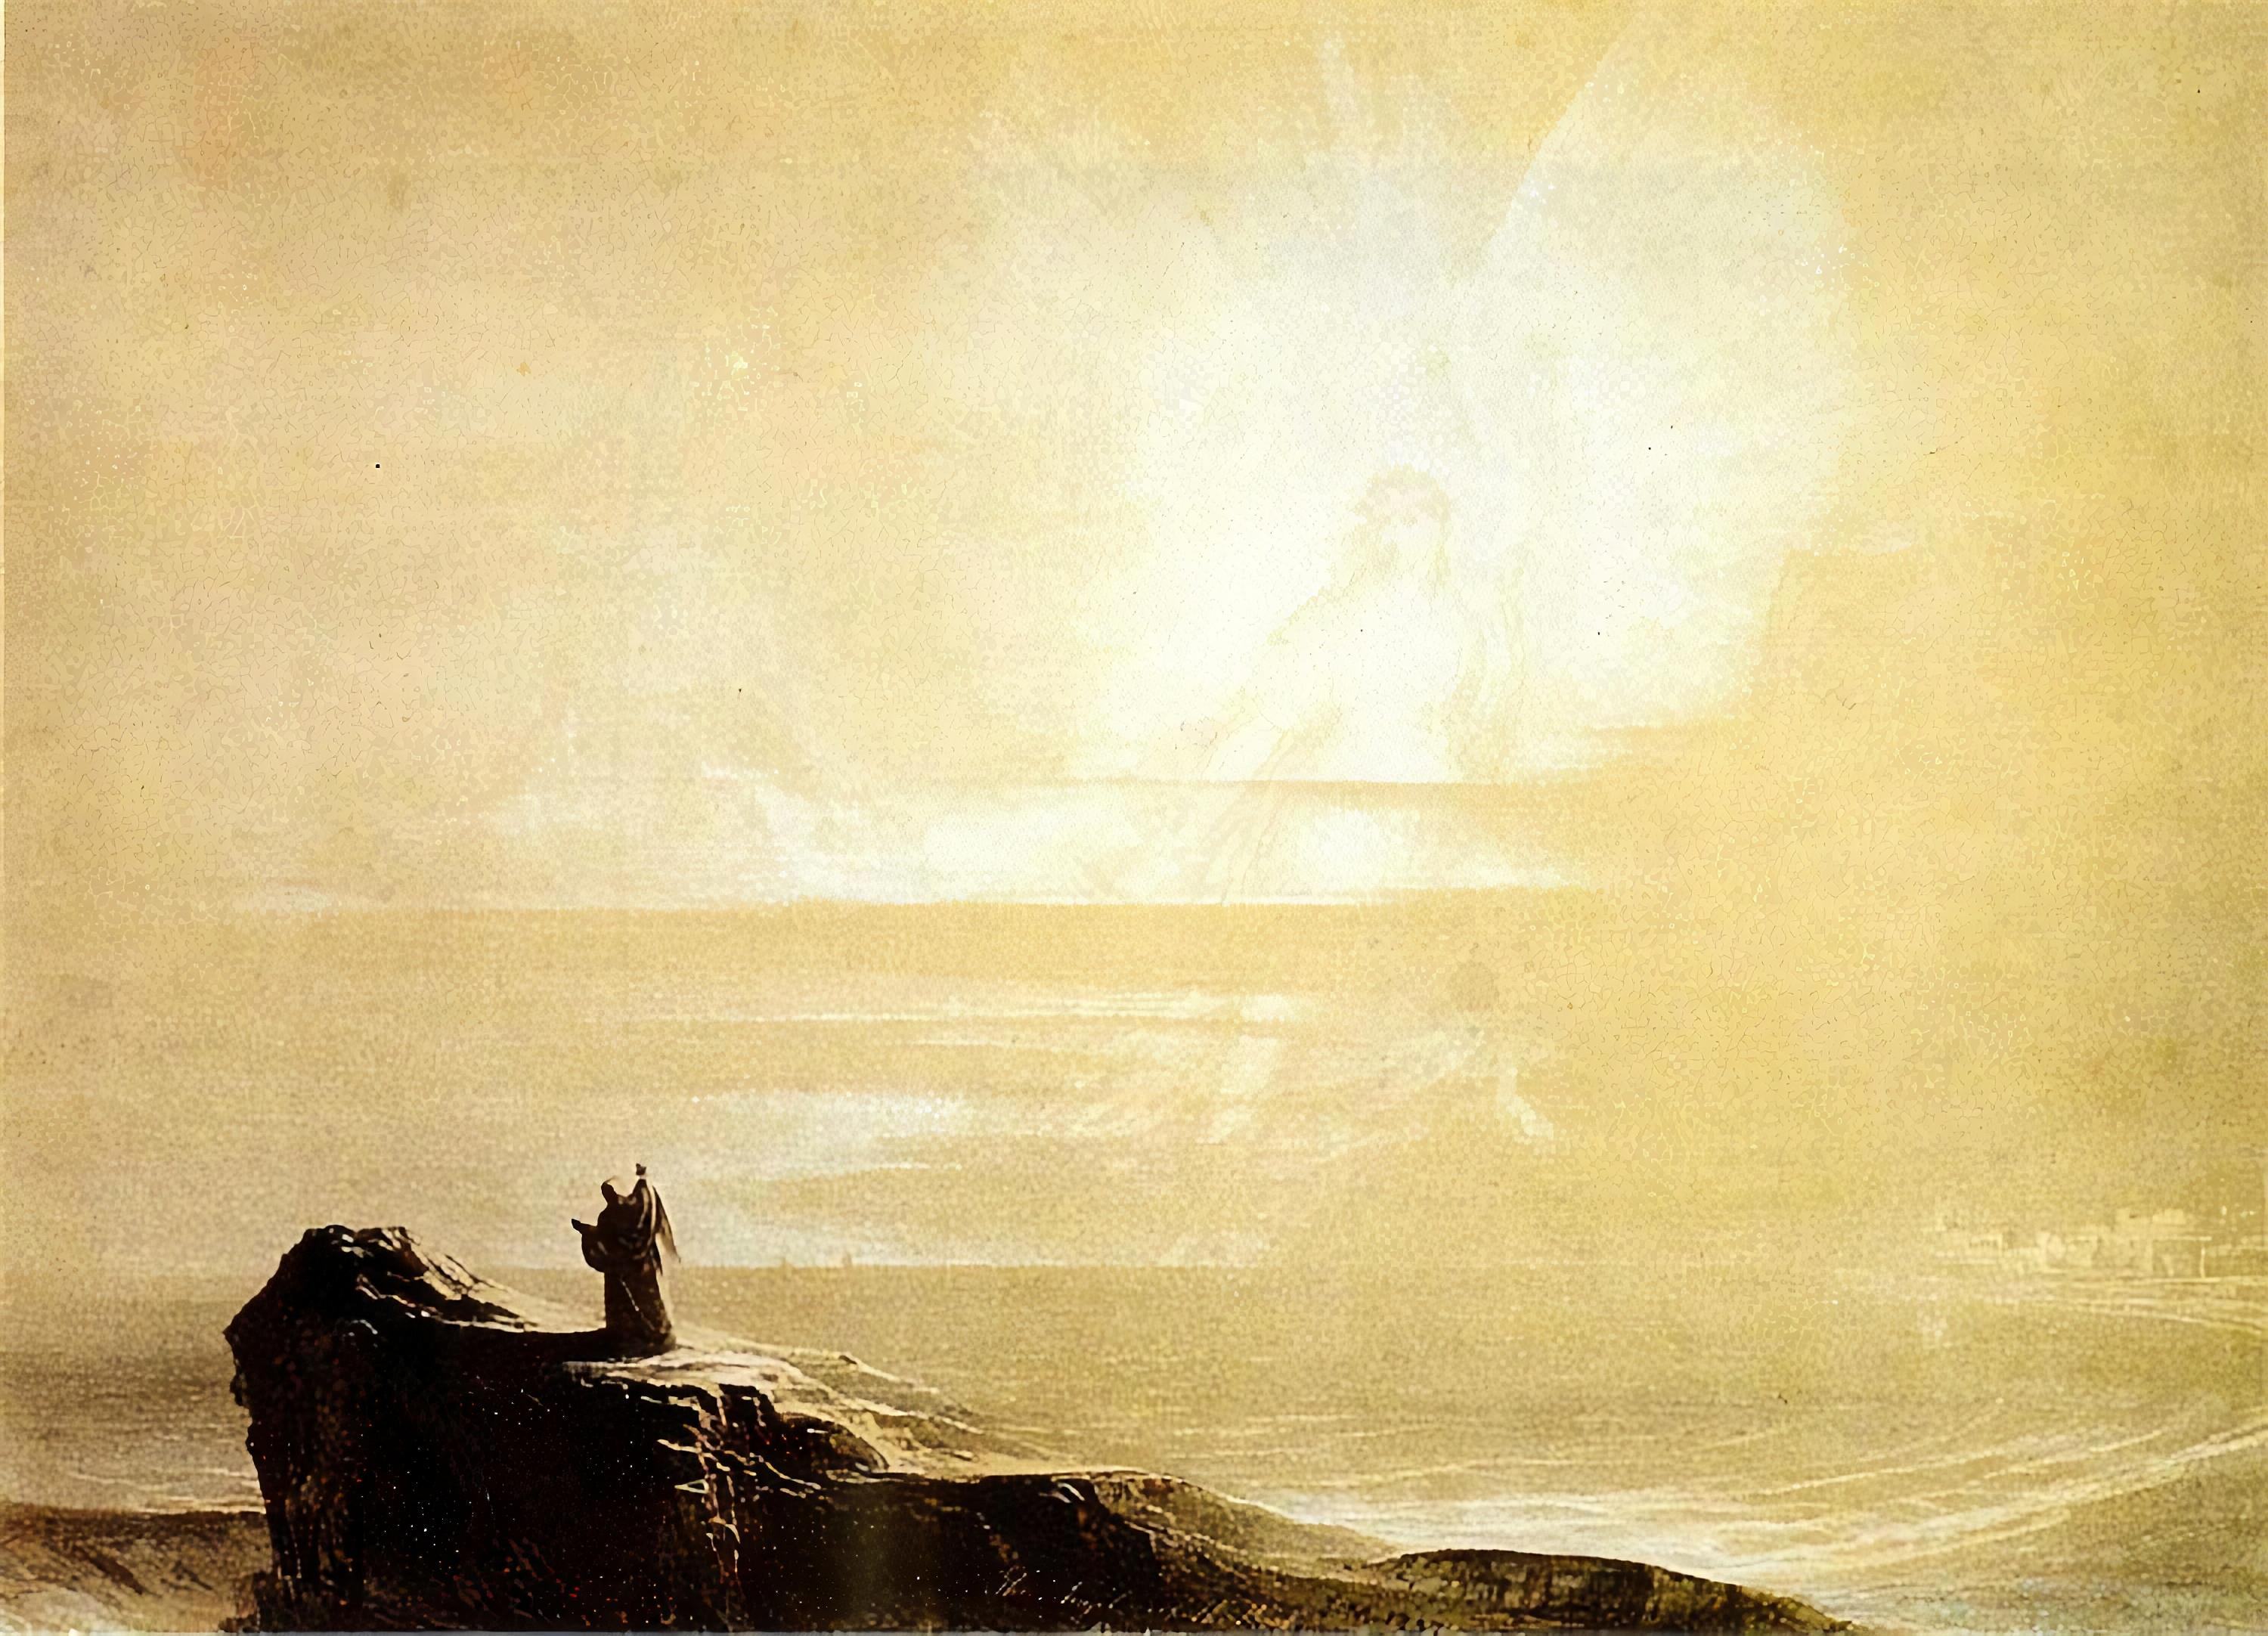
\includegraphics[angle=90, width=1\textwidth]{images/illustrations/johnmartinangelbook}
\end{center}